\documentclass[a4paper, 12pt]{report}
\usepackage{amsmath, amssymb}
\usepackage{tikz}

\begin{document}
	\begin{figure}[!hbt]
		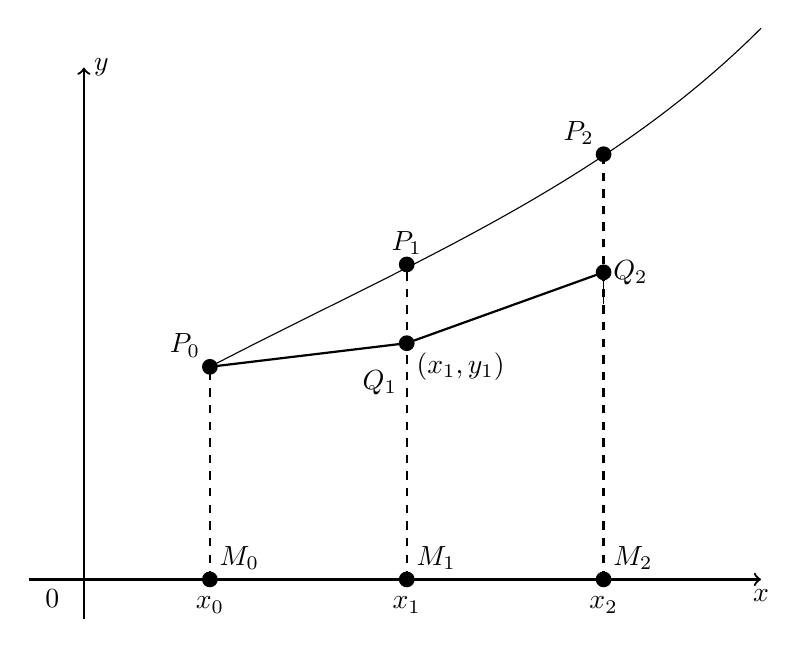
\begin{tikzpicture}
			%draw the basic lines  x and y coordinates
			\draw[thick, ->] (-0.3,0) -- (9,0) node[below]{$x$}; %x-axis
			\draw (0,0)--(0,0) node[below]{$0$}; %0 label
			\draw[thick, ->] (0.4,-0.5) -- (0.4,6.5) node[right]{$y$}; %y-axis
			
			%draw first dashes dots
			\foreach \x / \y in {2/2.7,4.5/3,4.5/4,7/3.9,7/5.4}
			\fill (\x,\y) circle(1mm);
			
			%first dashes dots labels
			\draw (2,2.7)--(2, 2.7) node[above left]{$P_0$};
			\draw (4.5,3)--(4.5, 3) node[below right]{$(x_1,y_1)$};
			\draw (4.5,4)--(4.5, 4) node[above]{$P_1$};
			\draw (7,5.4)--(7, 5.4) node[above left]{$P_2$};
			
			%draw the dashes
			\foreach \x / \y in {2/2.7,4.5/3,4.5/4,7/3.5,7/5.4}
			\draw[thick, dashed] (\x,0)--(\x,\y);
			
			%dashes labels
			\draw (4.5,2.5)--(4.5,2.5) node[left]{$Q_1$};
			\draw (7,3.5)--(7,3.9) node[right]{$Q_2$};
			
			%draw connectors 
			\draw[thick] (2,2.7)--(4.5,3); \draw[thick] (4.5,3)--(7,3.9);
			
			%draw the dashes dots on the line
			\foreach \x / \y in {2/0,4.5/1,7/2}
			\fill (\x,0) circle(1mm) node[above right]{$M_\y$};
			
			%dashes dots on  the line label down
			\foreach \x / \y in {2/0,4.5/1,7/2}
			\draw (\x,0)--(\x,-0.1) node[below]{$x_\y$};
			
			\draw (2,2.7) .. controls(4.5,4) and (7,5) .. (9,7);
		\end{tikzpicture}
	\end{figure}

	\begin{figure}[!hbt]
		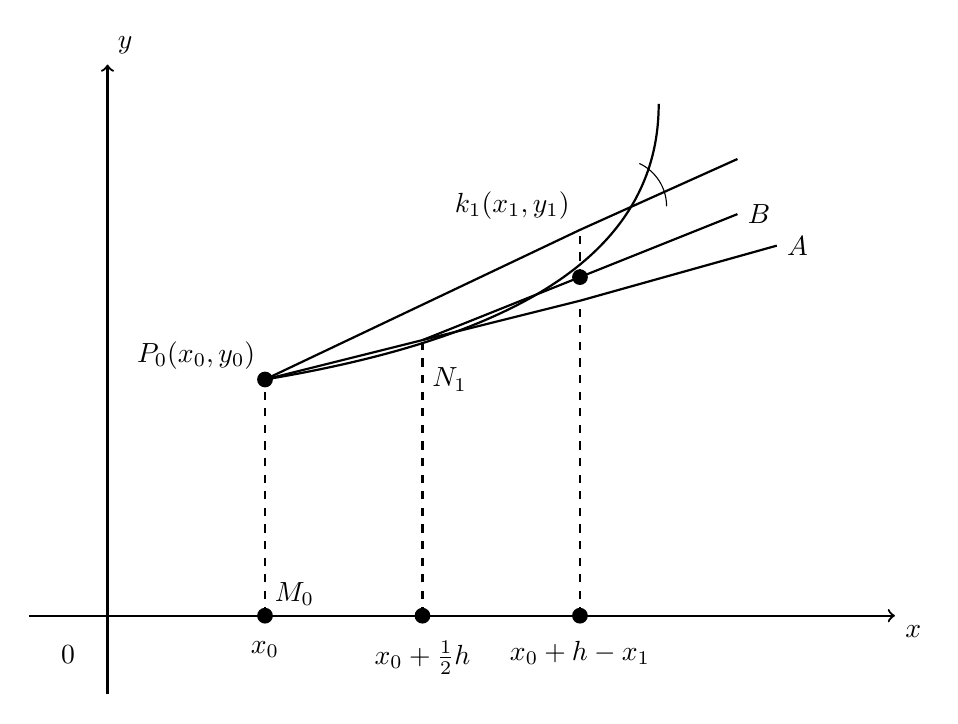
\begin{tikzpicture}
			\draw[thick, ->] (-1,0) -- (10, 0) node[below right]{$x$};
			\draw[thick, ->] (0,-1) -- (0, 7) node[above right]{$y$};
			\node[] (Z) at (-0.5,-0.5){$0$};
			
			\foreach \x in {2,4,6}
				\fill (\x,0) circle(1mm);
			
			\node[above right] at (2,0){$M_0$};
			\node[right] at (4,3){$N_1$};
			
			
			\node[below] at (2,-0.2){$x_0$};
			\node[below] at (4,-0.2){$x_0 + \frac{1}{2}h$};
			\node[below] at (6,-0.2){$x_0 + h - x_1$};
			
			
			\draw[dashed, thick] (2,0) -- (2,3);
			\fill (2,3) circle(1mm);
			\node[above left] at (2,3){$P_0(x_0,y_0)$};
			
			\draw[dashed, thick] (4,0) -- (4,3.5);
			
			\draw[dashed, thick] (6,0) -- (6,4);
			
			\fill (6,4.3) circle(1mm);
			\draw[dashed, thick] (6,4.3) -- (6,4.9)node[above left]{$k_1(x_1,y_1)$};
			
			\draw[thick] (2,3) -- (4,3.5) -- (6,4) -- (8.5,4.7) node[right]{$A$};
			
			\draw[thick] (4,3.5) --(6,4.3) -- (8,5.1)node[right]{$B$};
			
			\draw[thick] (2,3) --(6,4.9) -- (8,5.8);
			
			\draw[thick] (2,3) .. controls(5,3.5) and (7,4.5) .. (7,6.5);
			\draw (7.1,5.2) arc(0:65:6mm);
		\end{tikzpicture}
	\end{figure}

	\begin{figure}[!hbt]
		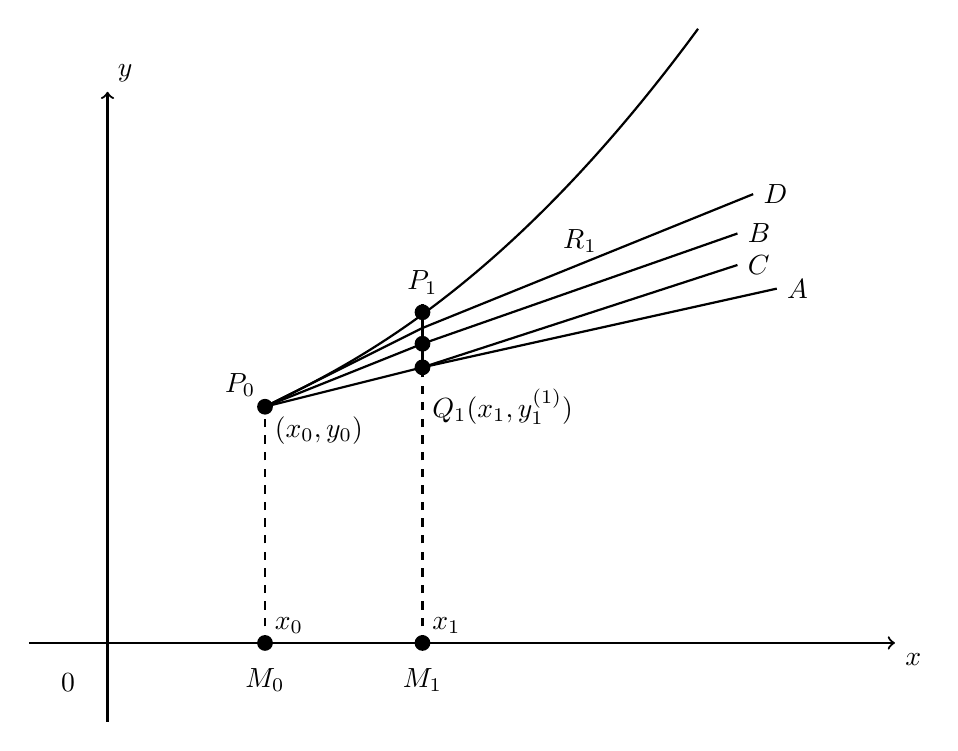
\begin{tikzpicture}
			\draw[thick, ->] (-1,0) -- (10, 0) node[below right]{$x$};
			\draw[thick, ->] (0,-1) -- (0, 7) node[above right]{$y$};
			\node[] (Z) at (-0.5,-0.5){$0$};
			
			\draw[dashed, thick] (2,0) -- (2,3);
			\fill (2,3) circle(1mm);
			\node[above left] at (2,3){$P_0$};
			\node[below right] at (2,3){$(x_0,y_0)$};
			
			\draw[dashed, thick] (4,0) -- (4,3.5);
			\fill (4,3.5) circle(1mm);
			\node[right] at (4,3){$Q_1(x_1,y_1^{(1)})$};
			\draw[thick] (2,3) -- (4,3.5)  -- (8.5,4.5) node[right]{$A$};
			
			\draw[thick] (4,3.5) -- (4, 3.8);
			\fill (4,3.8) circle(1mm);
			\draw[thick] (4,3.5) -- (8,4.8) node[right]{$C$};
			\draw[thick] (2,3) -- (4,3.8) -- (8,5.2) node[right]{$B$};
			\draw[thick] (2,3) -- (4,4) -- (8.2,5.7) node[right]{$D$};
			\node at (6,5.1){$R_1$};
			
			\draw[thick] (4,3.8) -- (4, 4.3) node[above]{$P_1$};
			\fill (4,4.2) circle(1mm);
			
			\draw[thick] (2,3) .. controls(3,3.5) and (5,4.4) .. (7.5,7.8);
			
			
			\node[above right] at (2,0){$x_0$};
			\node[above right] at (4,0){$x_1$};
			
			\foreach \x in {2,4}
				\fill (\x,0) circle(1mm);
			\node[below] at (2,-0.2){$M_0$};
			\node[below] at (4,-0.2){$M_1$};
						
		\end{tikzpicture}
	\end{figure}
\end{document}